\section{Hasil Eksperimen}\label{sec:results}
Entri bertanda \pending\ adalah eksperimen yang belum dijalankan; tidak ada nilai yang diperkirakan. Hasil yang tersedia saat ini hanya untuk TS2Vec dan berasal dari laporan kemajuan proyek. Metrik yang dipakai adalah AC@1 kecuali dinyatakan lain.

\subsection{C1: Kinerja RCA Antar Metode}
Tabel~\ref{tab:compare} adalah perbandingan C1 yang didefinisikan pada Bagian~\ref{sec:fair}.
\begin{table}
\caption{Perbandingan C1: kinerja RCA setiap metode pada konfigurasi terbaiknya yang dipilih pada kasus validasi (AC@1 dan AC@3 pada data uji, rata-rata dari 3 seed). RUN-encoder adalah varian adaptasi, bukan RUN asli. Semua sel masih terbuka sampai eksperimen dijalankan; nilai TS2Vec pada Tabel~\ref{tab:ex1} berasal dari konfigurasi tetap dan belum mengikuti aturan seleksi ini.}\label{tab:compare}
\centering
\small
\begin{tabular}{lcccc}
\toprule
 & \multicolumn{2}{c}{RE1} & \multicolumn{2}{c}{RE2}\\
\cmidrule(lr){2-3}\cmidrule(lr){4-5}
Metode & AC@1 & AC@3 & AC@1 & AC@3\\
\midrule
Chance level & \pending & \pending & \pending & \pending\\
Heuristik & 0,81 & \pending & 0,80 & \pending\\
RUN-original (tanpa transfer) & \pending & \pending & \pending & \pending\\
TS2Vec & \pending & \pending & \pending & \pending\\
TimeMAE & \pending & \pending & \pending & \pending\\
RUN-encoder & \pending & \pending & \pending & \pending\\
\bottomrule
\end{tabular}
\end{table}

\todo{Isi setelah eksperimen TimeMAE dan RUN selesai. Laporkan rata-rata $\pm$ SD dari 3 seed. Kerangka interpretasi: bandingkan metode hanya di dalam tabel ini; nyatakan anggaran tuning; jangan merangking metode dari hasil parsial.}

\subsection{EX-1: Pre-training dan Evaluasi In-domain}
Tabel~\ref{tab:ex1} melaporkan pre-training dan pengujian pada dataset yang sama.
\begin{table}
\caption{EX-1: AC@1 pada data uji, rata-rata $\pm$ SD dari 3 seed (pre-training dan pengujian pada dataset yang sama). Nilai TS2Vec berasal dari slide proyek; \pending\ menandai eksperimen yang belum dijalankan.}\label{tab:ex1}
\centering
\scriptsize
\setlength{\tabcolsep}{3pt}
\begin{tabular}{llccccc}
\toprule
 & & & \multicolumn{2}{c}{FineLast} & \multicolumn{2}{c}{FineAll}\\
\cmidrule(lr){4-5}\cmidrule(lr){6-7}
Dataset (kasus uji) & Metode & Heuristik & Pre-trained & Acak & Pre-trained & Acak\\
\midrule
RE1 (75) & TS2Vec  & 0,81 & 0,92$\pm$0,02 & 0,94$\pm$0,01 & 0,95$\pm$0,01 & 0,93$\pm$0,02\\
         & TimeMAE & 0,81 & \pending & \pending & \pending & \pending\\
         & RUN-encoder & 0,81 & \pending & \pending & \pending & \pending\\
\midrule
RE2 (45) & TS2Vec  & 0,80 & 0,89$\pm$0,02 & 0,86$\pm$0,01 & 0,86$\pm$0,01 & 0,87$\pm$0,02\\
         & TimeMAE & 0,80 & \pending & \pending & \pending & \pending\\
         & RUN-encoder & 0,80 & \pending & \pending & \pending & \pending\\
\midrule
RE3 (18) & TS2Vec  & 0,67 & 1,00$\pm$0,00 & 1,00$\pm$0,00 & 1,00$\pm$0,00 & 1,00$\pm$0,00\\
         & TimeMAE & 0,67 & \pending & \pending & \pending & \pending\\
         & RUN-encoder & 0,67 & \pending & \pending & \pending & \pending\\
\bottomrule
\end{tabular}
\end{table}

Pada TS2Vec, model hasil fine-tuning melampaui heuristik pada RE1 dan RE2 di keempat konfigurasi, dan encoder acak sama baiknya dengan encoder hasil pre-training pada sebagian besar sel; selisih terbesar antara pre-training dan acak adalah 0,03, setara satu atau dua kasus uji. Pada RE3, setiap konfigurasi mencapai 1,00. \todo{Tambahkan baris TimeMAE dan RUN-encoder setelah eksperimen dijalankan.}

\paragraph{Kontrol penghapusan anomali.} Data 240\,detik setelah injeksi diganti dengan salinan 240\,detik sebelum injeksi (Tabel~\ref{tab:anomaly}). AC@1 turun menjadi 0,03, 0,09, dan 0 pada RE1, RE2, dan RE3, jauh di bawah nilai aslinya. Hal ini menunjukkan bahwa model bergantung pada anomali dan tidak hanya pada identitas service. Slide melaporkan acuan tebakan acak sebesar $\pm$0,06; arti pastinya harus diklarifikasi sebelum dipakai sebagai chance level (Bagian~\ref{sec:metrics}).
\begin{table}
\caption{Kontrol penghapusan anomali (TS2Vec): AC@1 dengan data asli dan dengan jendela pasca-injeksi yang diganti salinan data pra-injeksi. Nilai berasal dari slide proyek, yang tidak menyebutkan konfigurasi model di baliknya.}\label{tab:anomaly}
\centering
\small
\begin{tabular}{lccc}
\toprule
Dataset & Data asli & Anomali dihapus & Tebakan acak (slide)\\
\midrule
RE1 & 0,91 & 0,03 & $\pm$0,06\\
RE2 & 0,9  & 0,09 & $\pm$0,06\\
RE3 & 1    & 0    & $\pm$0,06\\
\bottomrule
\end{tabular}
\end{table}


\subsection{EX-2: Transfer Lintas Dataset}
Tabel~\ref{tab:ex2} dan Gambar~\ref{fig:ex2} melaporkan RE2 sebagai target dengan mode FineLast, sedangkan Tabel~\ref{tab:bootstrap} melaporkan paired bootstrap terhadap encoder acak.
\begin{table}
\caption{EX-2: AC@1 pada RE2 (45 kasus uji) dengan FineLast, menurut persentase data latih berlabel, rata-rata dari 3 seed. Nilai TS2Vec dibaca dari grafik slide (dua desimal; SD tidak dilaporkan di sana). Pengaturan 10\% tidak memiliki nilai pada slide (``semua encoder setara''); tl = tidak dilaporkan. Heuristik memperoleh 0,80.}\label{tab:ex2}
\centering
\small
\begin{tabular}{llcccc}
\toprule
Metode & Encoder & 10\% & 25\% & 50\% & 100\%\\
\midrule
TS2Vec & Transfer dari RE1 & tl & 0,90 & 0,91 & 0,91\\
       & Transfer dari RE3 & tl & 0,86 & 0,88 & 0,87\\
       & In-domain (RE2)   & tl & 0,87 & 0,90 & 0,89\\
       & Acak              & tl & 0,84 & 0,84 & 0,86\\
\midrule
TimeMAE & Transfer dari RE1 / RE3, in-domain, acak & \pending & \pending & \pending & \pending\\
RUN-encoder & Transfer dari RE1 / RE3, in-domain, acak & \pending & \pending & \pending & \pending\\
\bottomrule
\end{tabular}
\end{table}

\begin{figure}
\centering
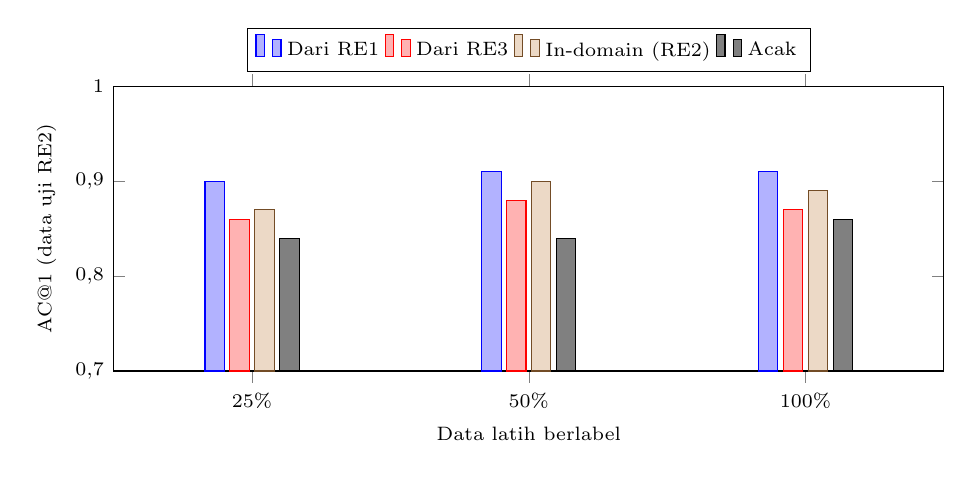
\begin{tikzpicture}
\begin{axis}[
  ybar, bar width=7pt, width=\textwidth, height=5.2cm,
  ymin=0.7, ymax=1.0, ylabel={AC@1 (data uji RE2)},
  yticklabel style={/pgf/number format/.cd, fixed, precision=1, use comma},
  scaled y ticks=false,
  symbolic x coords={p25,p50,p100}, xtick=data,
  xticklabels={25\%,50\%,100\%},
  xlabel={Data latih berlabel},
  legend style={at={(0.5,1.05)},anchor=south,legend columns=-1,font=\scriptsize},
  tick label style={font=\scriptsize}, label style={font=\scriptsize},
  enlarge x limits=0.25]
\addplot coordinates {(p25,0.90) (p50,0.91) (p100,0.91)};
\addplot coordinates {(p25,0.86) (p50,0.88) (p100,0.87)};
\addplot coordinates {(p25,0.87) (p50,0.90) (p100,0.89)};
\addplot coordinates {(p25,0.84) (p50,0.84) (p100,0.86)};
\legend{Dari RE1, Dari RE3, In-domain (RE2), Acak}
\end{axis}
\end{tikzpicture}
\caption{EX-2, TS2Vec, FineLast: AC@1 pada RE2 menurut fraksi data latih berlabel (nilai dari slide proyek, rata-rata 3 seed). Heuristik memperoleh 0,80 pada RE2; sumbu-y dimulai dari 0,7. Seri TimeMAE dan RUN-encoder akan ditambahkan ketika eksperimennya tersedia.}\label{fig:ex2}
\end{figure}

\begin{table}
\caption{Paired bootstrap (10.000 resampel) untuk selisih AC@1 antara encoder transfer dan encoder acak, hanya TS2Vec. Signifikansi sesuai pernyataan pada slide; interval kepercayaan hanya ditampilkan secara grafis di slide dan tidak direproduksi di sini.}\label{tab:bootstrap}
\centering
\small
\begin{tabular}{llcc}
\toprule
Target (sumber) & Pengaturan & Selisih & Signifikan\\
\midrule
RE2 (RE1) & FineLast 10\%  & 0,00 & tidak\\
          & FineLast 25\%  & +0,06 & ya\\
          & FineLast 50\%  & +0,07 & ya\\
          & FineLast 100\% & +0,05 & ya\\
          & FineAll 25\%   & +0,03 & tidak\\
          & FineAll 50\%   & +0,04 & ya\\
\midrule
RE1 (RE2) & FineLast 10\%  & 0,00 & tidak\\
          & FineLast 25\%  & $-$0,02 & tidak\\
          & FineLast 50\%  & $-$0,01 & tidak\\
          & FineLast 100\% & 0,00 & tidak\\
\bottomrule
\end{tabular}
\end{table}

Pada TS2Vec dengan RE2 sebagai target, encoder dari RE1 menghasilkan AC@1 sekitar 0,90--0,91 dengan 25\%--100\% label, dibandingkan 0,84--0,86 untuk encoder acak, dan selisihnya signifikan pada 4 dari 6 pengaturan yang dijalankan. Dengan 10\% label, semua encoder setara. Encoder dari RE3 tidak memberi manfaat. Dengan RE1 sebagai target, tidak ada encoder sumber yang memberi selisih signifikan.

\subsection{C2 dan C3: Pre-training, Label, dan Fine-tuning}
Tabel~\ref{tab:ex1}--\ref{tab:bootstrap} adalah bukti untuk kedua pertanyaan ini. Pada TS2Vec, FineAll tidak lebih baik daripada FineLast pada pengaturan yang dilaporkan. Untuk TimeMAE dan RUN-encoder, tabel yang sama dan Gambar~\ref{fig:ex2} akan diperluas, dan keuntungan terhadap encoder acak milik masing-masing metode adalah besaran yang dibandingkan antar metode.

\subsection{Metrik Tambahan}
\todo{AC@3 dan Avg@5 beserta chance level, setelah jumlah service per sistem diketahui dan kode metrik diterapkan pada semua metode.}
